\chapter{$W'$ y las anomalías en $R(D^{(*)})$}
\label{Ch:results}
Debido a que el decaimiento $b \to c \tau \nu$ está suprimido en el ME debido a la CKM(ver fig.~\ref{Fig:BW_decay}), es necesario obtener una nueva contribución a las corrientes cargadas para dar explicación a las anomalías en la medición de $R(D^{(*)})$. Una forma símple es extender el sector escalar del ME con un bosón gauge cargado $W^{\prime}$, el cual sólo se acopla a los fermiones de segunda y tercera generación, haciendo que sea más difícil la detección de este en el LHC. Además, la existencia de $\tau$’s en el estado final conduce a una dificultad, debido al background del ME en el LHC.

Debido a estas condiciones y el interés de esta investigación~\cite{Abdullah:2018ets} se propone que el $W'$ solo se acople a los quarks bottom ($b$) y charm ($c$) en el sector del color y a la tercera familia (sabor $\tau$) en el sector de leptones(ver fig.~\ref{Fig:BWp_decay}). Debido a que la probabilidad de encontrar un $b$ dentro del protón es muy baja, los canales de producción dominantes en este caso son la fusión $g g$ y $g c$, los cuales conducen a un jet $b$ asociado en el estado final. La presencia de este jet $b$ en el estado final da la posibilidad de diferenciar las señales del $W^{\prime}$ respecto al background del ME. Para esto se realiza un análisis exclusivo que requiere al menos un jet $b$ en estado final junto con un $\tau$ hadrónico y energía faltante, mejorando potencialmente la eficiencia de producción. Además, la existencia de un jet $b$ en estado final permitiría deducir la existencia de un acoplamiento a la tercera generación del $W^{\prime}$, lo cual es crucial para la explicación de las anomalías. 

Para comprender mejor la efectividad de esta técnica, contrastemos el uso del b-tags con reinterpretaciones de análisis inclusivos del $W^{\prime}$ realizados por ATLAS y CMS en los que no se hacen tales requisitos de jet $b$. En las Refs.~\cite{Khachatryan:2015pua, Aaboud:2018vgh}, la búsqueda inclusiva de $W^{\prime}$ se realiza sin referencia al mecanismo de producción y, por lo tanto, sin la necesidad del jet $b$. La Ref.~\cite{Altmannshofer:2017poe} considera el proceso $gc \to b \tau$ en el LHC, pero solo como un vértice efectivo y buscando decaimientos leptónicos de $\tau$ en lugar de hadrónicos. Sus resultados no son aplicables al rango de masas de interés en este trabajo. En Ref.~\cite{Asadi:2018wea} Se estudia un $W^{\prime}$ aparentemente idéntico al que se muestra aquí y los límites del colisionador se colocan solo de forma indirecta al reutilizar una búsqueda de ATLAS existente de un bosón gauge $Z^{\prime}$. Sus límites, aunque más concretos desde una perspectiva UV, dependen en gran medida del modelo. En Ref.~\cite{Dalchenko:2017shg}, se demuestra la importancia de los jets $b$ en las búsquedas de resonancias pero usando un bosón gauge $Z^{\prime}$ que decae en muones. Hay que destacar que, independientemente de las anomalías en los mesones $B$, las propiedades mencionadas anteriormente son dignas de investigación por si solas, además de servir como una pieza de rompecabezas adicional en el programa de búsqueda de resonancias en el LHC~\cite{Craig:2016rqv}.

Las interacciones que conectan la nueva física en este modelo con el ME están descritas por el siguiente Lagrangiano:
 %
 \begin{align}\label{Eq:LagWp}
 \mathcal{L} = ( g'_q \overline{c}  \gamma ^{\mu} P_{L} b +g'_{\tau} \overline{\nu}_{\tau}  \gamma ^{\mu} P_{L} \tau^{-}){W^{\prime}}_{\mu}^{+} + h.c.\,,
 \end{align}
 %
donde $g^{\prime}_{q}$ y $g^{\prime}_{\tau}$ son los acoples de nueva física. Debido a que estos acoplamientos violan sabor, construir una afinación UV que sea consistente con el ME no es sencillo. Un ejemplo de tal afinación UV se da en~\cite{Boucenna:2016qad} , donde se supone que el $W^{\prime}$ solo se acopla directamente a una generación de fermiones vector-like demasiado pesados para ser observados. Los acoplamientos en Eq.~\eqref{Eq:LagWp} luego se inducen a través de mezclas entre los nuevos fermiones y los fermiones del ME. En cualquier modelo UV de este tipo, se hacen muchas suposiciones adicionales que deben probarse individualmente en comparación con el experimento, y rara vez se puede descartar todo el espacio de posibles modelos. Por lo tanto, en lugar de demostrar la viabilidad de esta instancia particular de tales modelos, adoptamos el enfoque pragmático de referirnos al mecanismo en~\cite{Boucenna:2016wpr} como una prueba de principio y centrarnos en cambio en las implicaciones del colisionador sobre un constructo mínimo.
%
\begin{figure}
\begin{center}
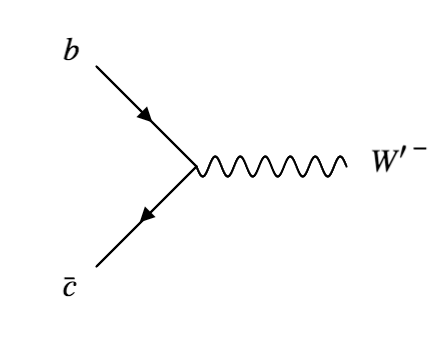
\includegraphics[width = 0.28 \textwidth]{diag_bc.png}
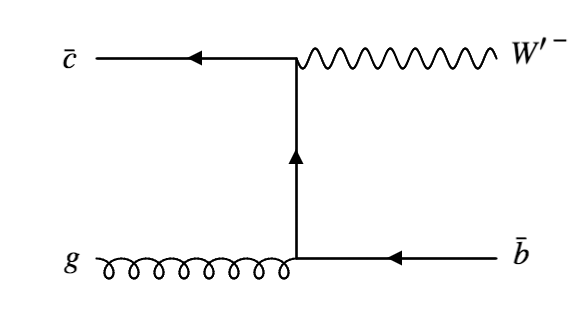
\includegraphics[width = 0.35 \textwidth]{diag_gc.png}
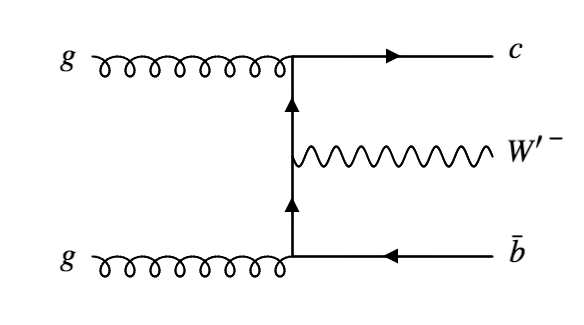
\includegraphics[width = 0.35 \textwidth]{diag_gg.png}
\caption{Representación de diagramas de Feynman de producción de $W'$ en el LHC.}
\label{Fig:diag}
\end{center}
\end{figure}
%

Los principales canales de producción del $W^{\prime}$ en el LHC se muestran en la Fig.~\ref{Fig:diag}. La producción a través de cualquier otro estado inicial se suprime por medio de acoplamientos adicionales. Para acoplamientos y número de estados finales mayores las contribuciones en sección transversal de estos diagramas estarían ordenados de izquierda a derecha. Esto se contrarrestaría con la diferencia en la fracción de momento transportada por gluones, quarks $c$  y quarks $b$. Uno esperaría que los diagramas con gluones en el estado inicial sean dominantes. Como se vera, la eficiencia del requisito del b-tags sugiere que esto es cierto en buena medida.

Debido a que el rango de masas que se toma en cuenta está por encima de los $200$ GeV, todos los productos de los decaimientos son no masivos, lo cual ayuda a simplificar las expresiones para los branchings, los cuales se pueden calcular de la Eq.~\eqref{Eq:Branching}:
%
\begin{align}
B({W'}^+ \to \tau^+\nu_{\tau}) \approx& \frac{|g'_{\tau}|^2}{|g'_{\tau}|^2+3 |g'_q|^2}\,, &
B({W'}^+ \to c\bar{b} ) \approx& \frac{3 |g'_{q}|^2}{|g'_{\tau }|^2+3 |g'_{q}|^2}\,.
\end{align}
%
Siguiendo~\cite{Boucenna:2016qad}, los observables van a estar dados por:
%
\begin{align}
R(D^{(*)})_{\text{NF}} = \left( 1 + \frac{g'_{\tau}g'_q}{m^2_{W'}} \frac{\sqrt{2}}{4 G_F V_{cb}}\right)^2 R(D^{(*)})_{\text{ME}}\,,
\end{align}
%
donde $m_{W'}$ es la masa del bosón $W'$, $G_F = 1.16 \times 10^{-5}$ GeV$^2$ es la constante de Fermi, y $V_{cb} = 0.04$ es la componente $cb$ de la matriz CKM. Definiendo los nuevos acoples positivos, el valor central para $R(D)$ y $R(D^{*})$ requieren que el factor $g'_qg'_{\tau}/m^2_{W'}$ sea igual a $0.002(100\text{ GeV}/m_{W'})^2$ y $0.001(100\text{ GeV}/m_{W'})^2$ respectivamente. En este estudio se presentan límites en el plano $m_{W'}-g'_q$ para diferentes valores de $g'_{\tau}$.

\section{Coordenadas en los detectores}
Cada detector en un acelerador está hecho para cubrir un determinado ángulo solido dependido de lo que se quiera estudiar. Dentro del ángulo sólido elegido de un experimento, ninguna partícula debe escapar de la detección, excepto por los neutrinos, los cuales debido a su interacción débil no interactúan en la escala de longitud de un detector típico. Todas éstas partículas que escapan del detector son conocidas como energía transversa faltante $E^{\text{miss}}_T$.

El sistema de coordenadas en los detectores del LHC se definen de la siguiente manera: 
El punto de interacción se define como el origen del sistema de coordenadas. El eje $z$ corre a lo largo de la línea del haz. El plano $x$ - $y$ es perpendicular a la línea del haz y se conoce como el \textquotedblleft plano transversal\textquotedblright. El eje $x$ positivo apunta desde el punto de interacción al centro del anillo principal del LHC; el eje $y$ positivo apunta hacia arriba de la superficie de la Tierra. En el caso de los detectores cilíndricos, aprovechando su simetría, se utilizan coordenadas cilíndricas. En general el plano transversal se describe en términos de las coordenadas $r$ - $\phi$. El ángulo azimutal $\phi$ se mide desde el eje $x$, alrededor del haz, y el radio $r$, es la longitud desde la línea del haz. El ángulo polar $\theta$ se cuenta desde el eje $z$ positivo. El ángulo polar a menudo también se da en términos de la pseudorapidez, definida como $\eta = -\ln \tan (\theta/2)$.
La pseudo-rapidez es la aproximación sin masa de la variable de rapidez $y$ definida para una partícula con energía $E$, momento $p$ y momento longitudinal $p_L = | p | \sin \theta$ a lo largo del haz como
%
\begin{align*}
y = \frac{1}{2}\ln \frac{E+p_L}{E-p_L} \approx \eta = \frac{1}{2}\ln \frac{|p|+p_L}{|p|-p_L} = -\ln \tan\left( \frac{\theta}{2} \right)\,.
\end{align*}
%
Se usa la pseudorapidez $\eta$ en lugar del ángulo polar porque los detectores son cilindros concéntricos, lo que limita los ángulos polares en los que se obtiene una reconstrucción precisa de la energía transversa $E_T$, de las partículas. Por otra parte, la producción de partículas es aproximandamente, constante en función de $\eta$.

En este sistema de coordenadas en lugar de utilizarse el modulo del momento, se utiliza el momento transverso $p_T$, el cual se define como la componente del momento en el plano transversal $p_T = | p | \cos \theta$. Esta cantidad es importante, ya que es posible calcularla a partir de la $E_T$, depositada en los calorímetros en los detectores.

Señales de nueva física en un colisionador puede ser detectadas mediante el decaimiento del $W^{\prime}$ a un $\tau_h$ y $E^{\text{miss}}_T$. Estas señales pueden ser vistas como una característica en el espectro observado de masa transversal, definido como
%
\begin{align*}
M_{T} = \sqrt{2p^{\tau}_{T} E^{\text{miss}}_{T}(1-\cos [\Delta \phi (p^{\tau}_{T},p^{\text{miss}}_{T})])}\,,
\end{align*}
%
donde $p^{\tau}_{T}$ es la magnitud del vector momento transversal del candidatos a $\tau_h$, $\Delta \phi$ es la diferencia en el ángulo azimutal entre $p^{\tau}_{T}$ y $E^{\text{miss}}_{T}$ y $E^{\text{miss}}_T$ es el modulo de $\vec{p}^{\text{miss}}_{T}$, el cual se define como $-\sum_{i} \vec{p}_{T}$ de todas las partículas que no interaccionan con el detector. Debido a que los decaimientos hadrónicos del lepton $\tau_h$ se pueden diferenciar experimentalmente, debido a su baja multiplicidad de hadrones cargados, a diferencia de los jets que se originan de la hadronización de partones producidos en el proceso de dispersión dura, que tienen alta multiplicidad de hadrones cargados, por lo que $m_{T}$ podría usarse para identificar las resonancías del $W^{\prime}$.

Otra cantidad importante para la reconstrucción de los eventos en el detector es la distancia angular, la cual es definida como $\Delta R = \sqrt{(\Delta \eta)^2+(\Delta \phi)^2 }$.

\section{Muestras y simulaciones}

La producción del par de quarks ($t\bar{t}$) con jets asociados de estados iniciales de radiación (EIR), comunmente referido a un evento semileptónico $t\bar{t}+$jets, donde $t\bar{t} \to b W^+ \bar{b}W^- \to b\bar{b}\ell^{\pm}\nu_{\ell}q\bar{q}$, representa la fuente dominante de background ($61\%$ de el background total). La siguiente fuente de background, 21\%, viene de la producción de un bosón $W$ con jets de EIR ($W+$jets), donde se produce un leptón real de un $W$ y la energía transversal faltante ($E^{\text{miss}}_T$) es obtenida del neutrino asociado del decaimiento del $W$. Los producción de eventos de Drell-Yann (DY) ($Z/\gamma^*$), más un jet de EIR, contribuyen al $11\%$ del background total. El decaimiento leptónico del bosón $Z/\gamma^*$ entrando en los estados finales de los eventos seleccionados cuando uno de los leptones se pierde en la reconstrucción, dando lugar a la energía transversal faltante. Otras contribuciones al background provienen de los eventos con un solo quark top y la producción de pares vectoriales ($WW$, $ZZ$, $WZ$), referidos como un evento dibosónico, más jets de EIR. La señal simulada y el background se calcula a orden principal (LO de las siglas en inglés). Esto fueron producidos usando \textsc{MadGraph} (v.2.6.0)~\cite{Alwall:2014hca} interconectado con \textsc{PYTHIA 8} \cite{Sjostrand:2014zea} para la hadronización de partones y \textsc{DELPHES} (v3.3.2)~\cite{deFavereau:2013fsa} fue usado para incluir la interacción de partículas con el detector (se usaron las tarjetas de configuración de CMS). El modelo fue implementado usando \textsc{FeynRules 2.3}~\cite{Christensen:2008py,Degrande:2011ua,Alloul:2013bka}.

Para los eventos de la señal, los procesos de matching y merging fueron implementados usando el algoritmo MLM~\cite{Alwall:2007fs}. Los parámetros de matching, \textbf{xqcut} y \textbf{qcut} se verificaron para que el resultado de la sección transversal sea razonablemente estable, además posea una transición suave en la taza de distribución diferencial de jets entre los eventos con $N$ y $N + 1$ jets, pero no se optimizaron aún más debido a los problemas inherentes en el modelado de las emisiones de quarks pesados. La variable \textbf{xqcut} define la distancia mínima entre partones en el nivel MadGraph, mientras que la variable \textbf{qcut} establece la dispersión mínima de energía para un jet agrupado en PYTHIA. Para la producción de señal, se usaron \textbf{xqcut} de $30$ y \textbf{qcut} de $60$ donde se uso un valor de 5 para el parámetro \textquotedblleft jet flavor scheme\textquotedblright.

Hay que tener presente que hay una gran incertidumbre sistemática en el proceso de matching que no tenemos en cuenta. Esta incertidumbre es mayor cuando los diagramas de mayor multiplicidad (los dos diagramas de la derecha de la figura~\ref{Fig:diag} se descartan aunque la sección transversal correspondiente no cambie). No esperamos que la incertidumbre afecte la eficiencia de selección de los jets duros que necesitamos, aunque la sección transversal total podría en realidad ser mayor o menor hasta en un $30\%$. Esto modifica la sensibilidad proyectada absoluta, pero la comparación entre el análisis exclusivo e inclusivo sigue siendo válida.

Otra posible fuente de error son las divergencias colineales a altas masas de $W'$ en el segundo y tercer diagrama (Fig.~\ref{Fig:diag}), los cuales pueden arruinar la validez del cálculo perturbativo. Una forma de evitar esto es restringir el valor de corte de $p_T$ del $b$-jet como se prescribe en \cite{Degrande:2016aje}. Alternativamente, podemos simular los eventos en NLO con una cascada de partones adecuada para extender el dominio de validez de nuestro corte de $p_T$. Siguiendo el procedimiento utilizado por \cite{Fuks:2017vtl} generamos archivos del modelo compatibles con los cálculos de NLO utilizando \textsc{FeynRules 2.3} \cite{Degrande:2014vpa} y producimos muestras para compararlas con los resultados LO. Encontramos que la sección transversal aumenta aproximadamente un 15\% para una masa del $W'$ de 200 GeV y aproximadamente un 7\% para una masa del $W'$ de 1 TeV para NLO en comparación con LO, mientras que cualquier alteración en la distribución $b$-jet $p_T$ es insignificante (ver apéndice \ref{LOvsNLO}). Usamos los resultados LO para establecer nuestra sensibilidad teniendo en cuenta que los resultados de NLO mejorarían nuestro alcance.

Las simulaciones son afectadas por las incertidumbres asociadas con la generación de los eventos, la simulación del detector y la determinación de la luminosidad integrada. La incertidumbre en la luminosidad integrada es de $2.6\%$~\cite{CMS-PAS-LUM-13-001}. La incertidumbre en la escala de energía del $\tau$ es del $3\%$ para eventos con bajo $p_{T}$~\cite{Khachatryan:2015dfa}. La escala de energía de los jets tiene una incertidumbre entre $3\%$ y $5\%$, dependiendo del $p_{T}$ y el $\eta$~\cite{Khachatryan:2016kdb}. La probabilidad de clasificar un electrón como un $\tau_h$  es de $3-14\%$~\cite{ATLAS-CONF-2017-029}. La incertidumbre en $E^{\text{miss}}_{T}$ es despreciable para $E^{\text{miss}}_{T} > 300$ GeV y del $10\%$ aproximadamente para $E^{\text{miss}}_{T} < 300$ GeV~\cite{Aaboud:2018vgh}.

Gran parte de las mediciones que se realizan en los experimentos de física de altas energías se definen como ejercicios de conteo (determinar cuantos son los eventos de un proceso especifico), por lo que se describen con la estadística de Poisson. La estadística de Poisson se define como al probabilidad de que ocurran una cantidad determinando de eventos en un cierto periodo de tiempo. Ésta estadística se especializa en la ocurrencia de sucesos de baja probabilidad, lo que la hace optima para describir los eventos de señal ($W^{\prime}$) en comparación con los eventos de background (SM). En una distribución de Poisson, la varianza es igual a $N$, por lo tanto, la desviación estándar es $\sigma = \sqrt{N}$.

Para los datos simulados, podemos encontrar eventos de señal ($S$) y eventos de background (B), por lo que el número total de eventos estará dado por $N = S + B$. La significancía es la probabilidad de que al realizar un experimento, éste rechace la hipótesis incial (ME) , dado que era cierta. Por lo que se puede definir la significancia de la señal como el tamaño de la señal en relación con el error del total de los eventos ($\sigma$), es decir, $S/\sqrt{S+B}$. Esto permite dar cuenta del error de todos los eventos, a diferencia de la definición  de significancia $S/ \sqrt{B}$, la cual solo toma en cuenta el background, por lo que podría sobre estimar la significancia de la señal~\cite{Punzi:2003bu}

\textbf{Nota:} Los archivos del modelo en \textsc{FeynRules}, las \textquotedblleft process cards\textquotedblright para \textsc{MadGraph}, y el notebook de \textsc{Mathematica} usados para este estudio se pueden encontrar en~\cite{mo_abdullah_2018_1240452}. Para propositos de reproducibilidad, utilidad y revisión de pares. Igualmente, los resultados fueron publicados en arXiv:1805.01869 [hep-ph]~\cite{Abdullah:2018ets}

\section{Análisis}\label{sec:Analysis}
%
\vspace{10 pt}
\begin{table}
\begin{center}
\begin{tabular}{ l  c}\hline\hline
Criterio & Selección\\
 \hline
    $N_{\tau_{h}}$       & $\ge$ 1 \\
    $|\eta_{\tau_{h}}|$ & $< 2.3$ \\
    $p_{T} (\tau_{h})$ & $> 80$ GeV \\
    Veto second $\tau_{h}$ &  $> 50$ GeV \& $|\eta_{\tau_{h}}| < 2.3$ \\
    $N_{e/\mu}$ with $p_{T} > 15$ GeV & $= 0$ \\
    $N_{b-\text{jets}}$ & $= 1$\\
    $p_{T} (b-\text{jets})$ & $> 20$ GeV \\
    $|\eta_{b-\text{jets}}|$ & $< 2.5$ \\
    $ E^{\text{miss}}_{T}$ & $> 140$ GeV \\
     $|\Delta \phi (\tau_{h}, E^{\text{miss}}_{T})|$ & $ > 2.4$ \\
   \hline\hline
 \end{tabular}
 \caption {Criterios de selección de eventos usados para el análisis.}
 \label{tab:selections}
\end{center}
\end{table}
%

El decaimiento hadronico del $\tau$ está compuesto de un neutrino y un conjunto de hadrones cargados (típicamente uno o tres piones cargados y hasta dos piones neutros)~\cite{Aad:2014rga}. Lo cual permite diferenciar los $\tau_h$ de los diferentes jet en el proceso. Ya que el análisis requiere al menos un $\tau$ hadrónico de estado final, para identificar un jet como uno $\tau_h$, este debe tener un $p_T > 80$ GeV y $|\eta_{\tau_h}| < 2.3$ para que estén dentro de la región de aceptación del tracker. Eventos con un candidato $\tau_h$ adicional con $p_T > 50$ GeV y $|\eta_{\tau_h}| < 2.3$ fueron prohibidos, lo cual ayuda a reducir las contribuciones de dibosón y DY+jets. Además, en esta parte del espacio de parámetros la eficiencia de identificación y la tasa de identificación de fallas son aceptables~\cite{Padeken:2265826}. 

De las topologías en la fig.~\ref{Fig:diag}, se establece que un jet con $p_T > 20$ GeV y $|\eta_{\tau_h}| < 2.5$ identificados como un quark $b$ sea seleccionado. Ya que al subir el $p_T$ del jet por encima de 20 GeV trae una mejora en la resolución,  por lo que dicho valor se establece como el mínimo $p_T$ para seleccionar un jet~\cite{ATL-PHYS-PUB-2015-023}. 
%
\begin{figure}
\begin{center}
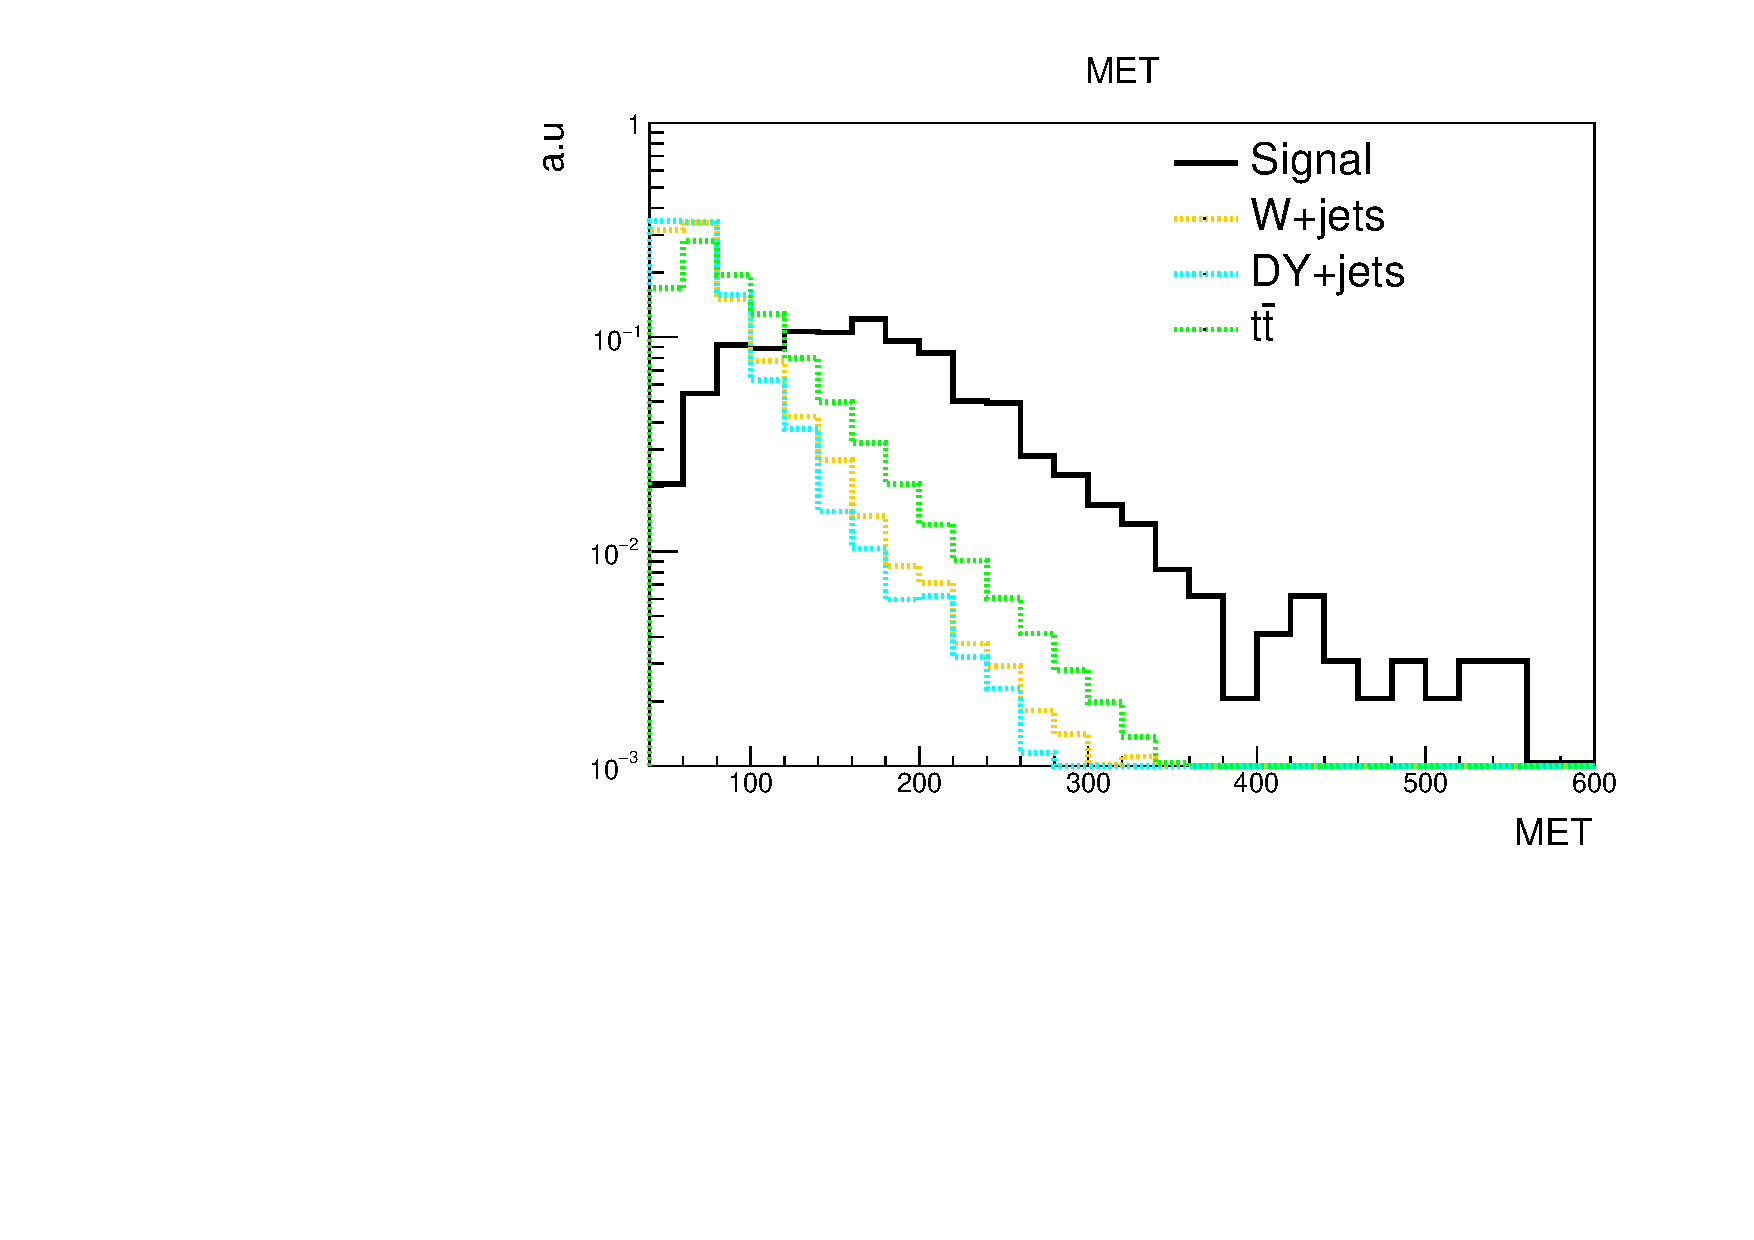
\includegraphics[width = 0.45 \textwidth]{figures/Wp_MET}
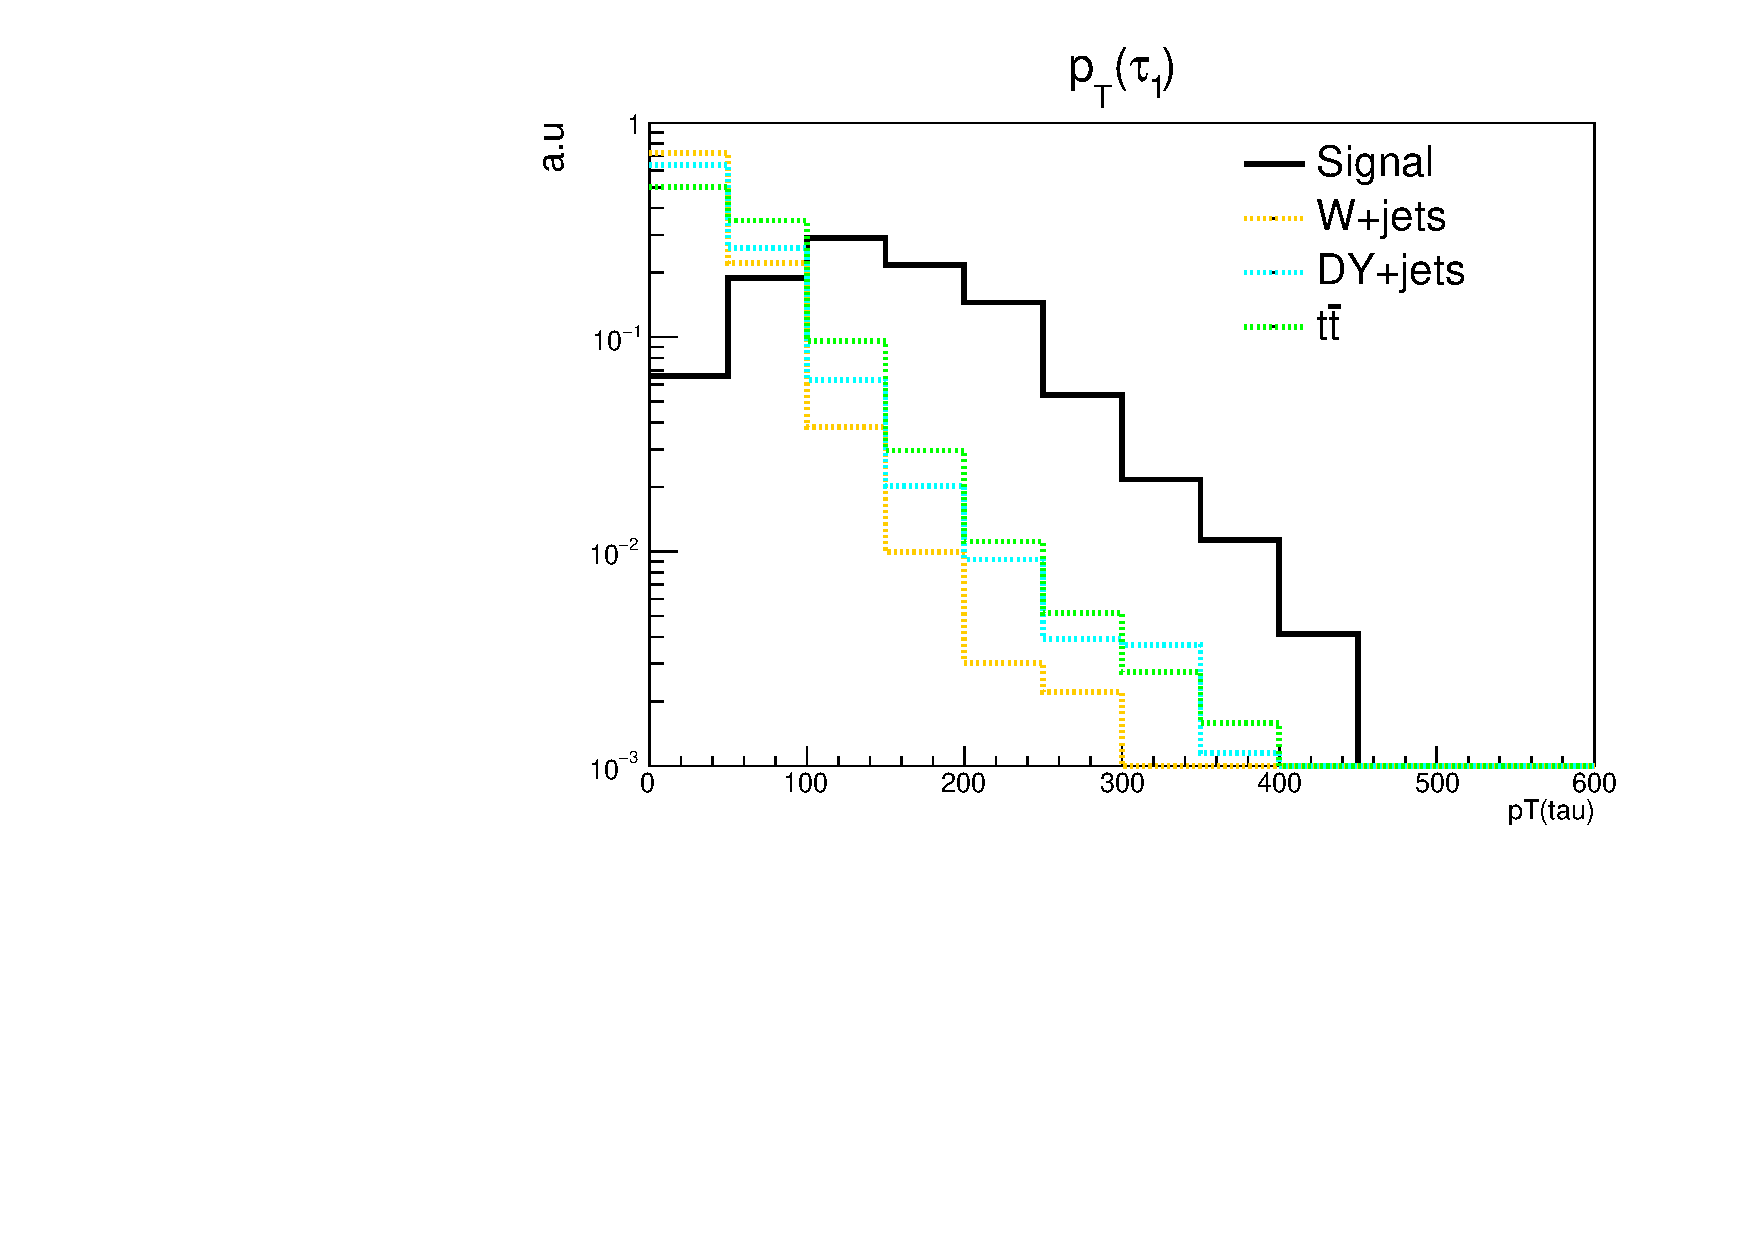
\includegraphics[width = 0.45 \textwidth]{figures/Wp_Tau_pT}
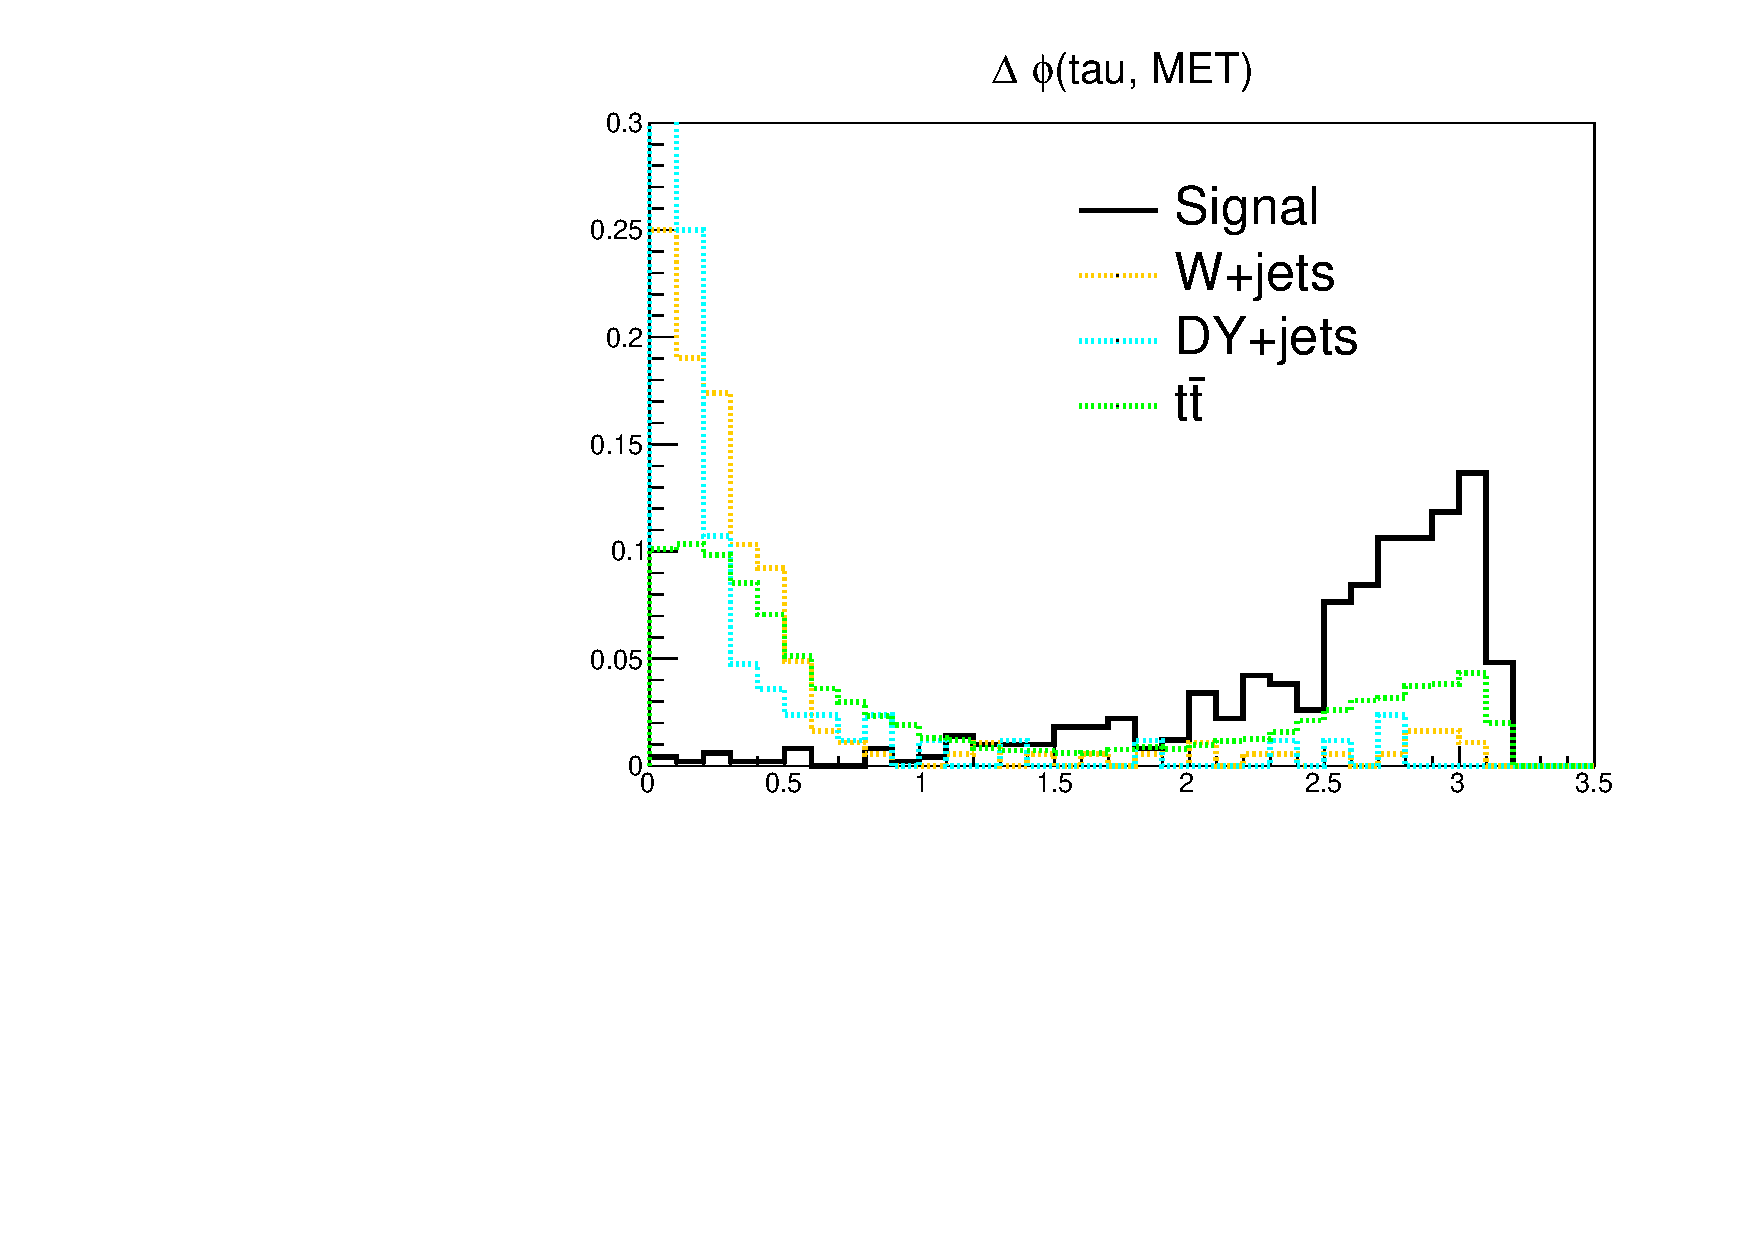
\includegraphics[width = 0.45 \textwidth]{figures/Wp_Delta_phi}
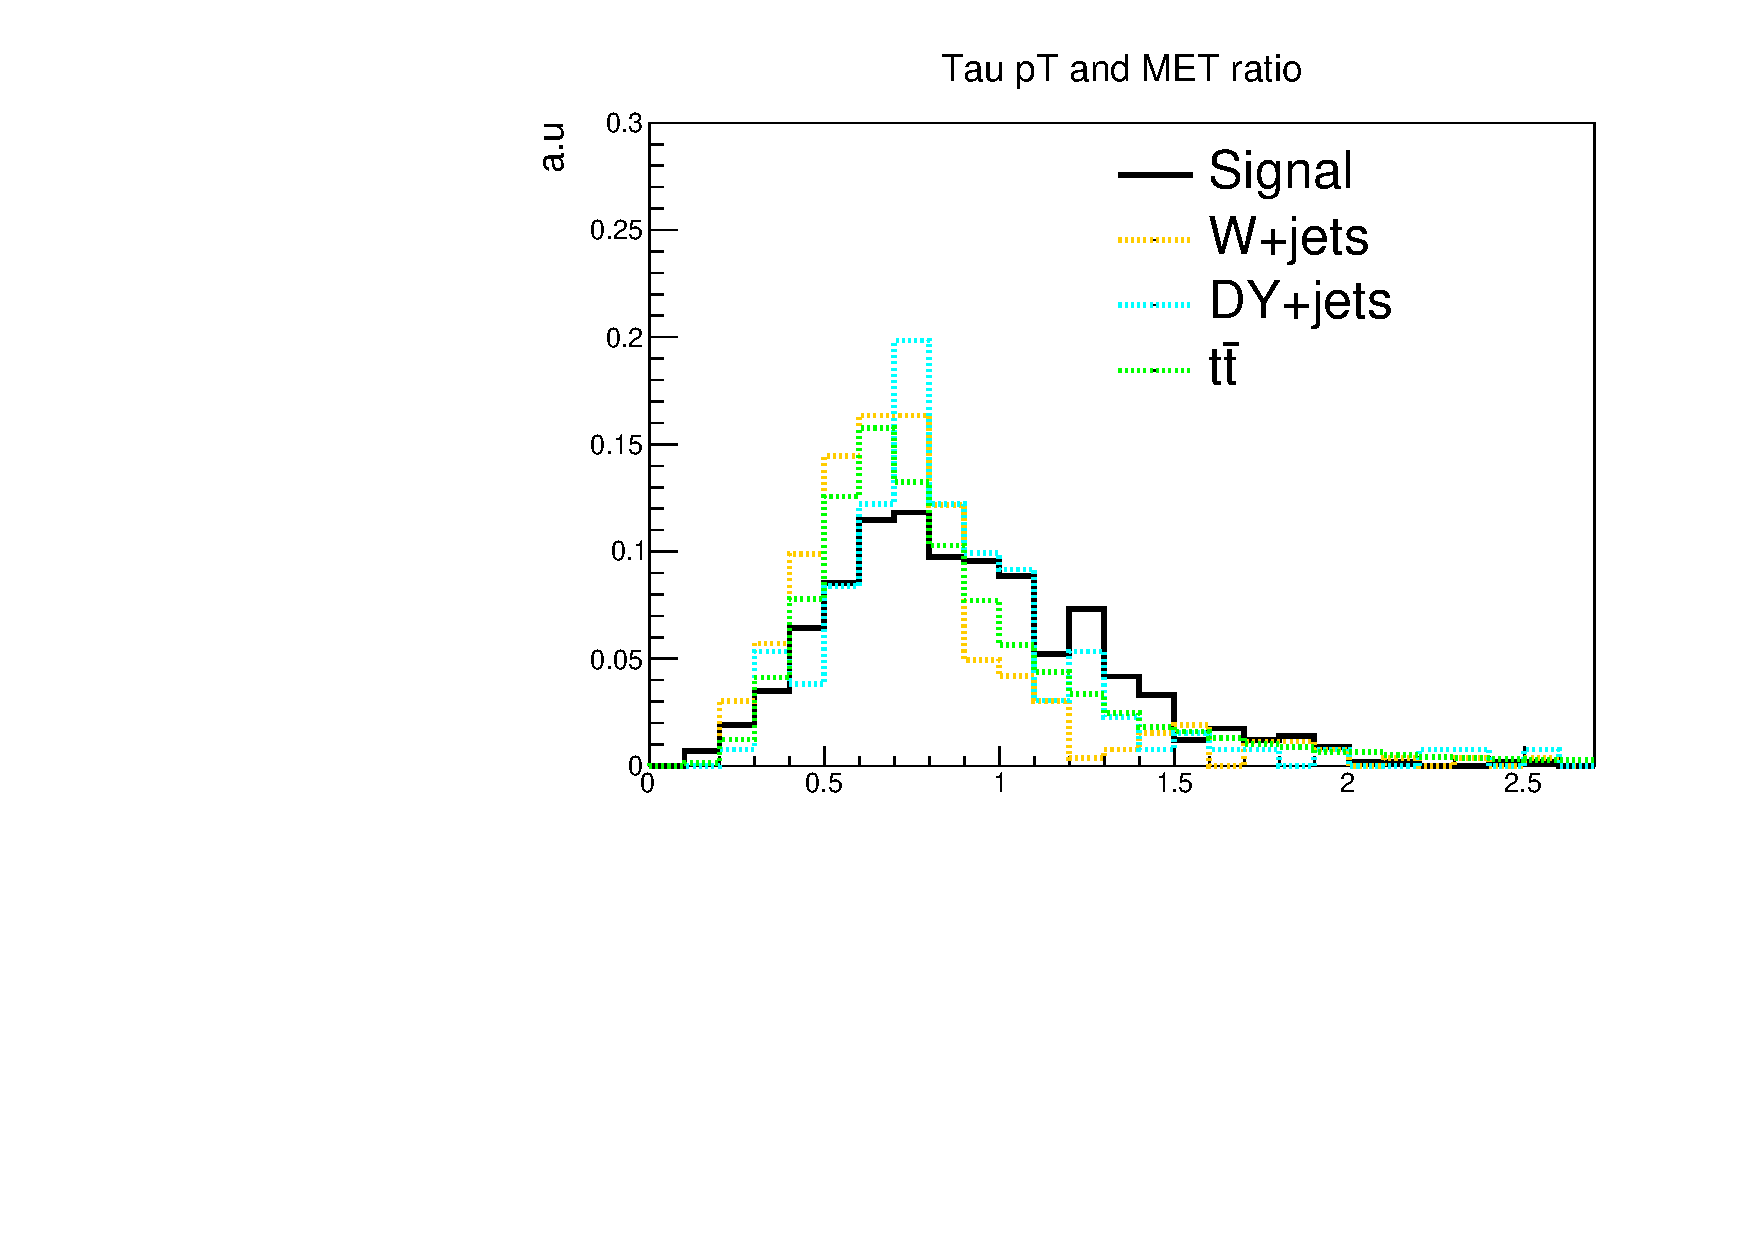
\includegraphics[width = 0.45 \textwidth]{figures/Wp_TauPt_MET_ratio}
\caption{En el grafico se comparan las siguientes distribuciones cinemáticas: $E^{\text{miss}}_{T}$ (superior izquierda), $p^{\tau}_{T}$ (superios derecha) y $\Delta \phi (p^{\tau}_{T}, E^{\text{miss}}_{T})$ (inferior izquierda) y $p^{\tau}_{T}/E^{\text{miss}}_{T}$ (inferior derecha). Para una señal con $M_{W^{\prime}}=500$ GeV y $g_{\tau}=g_{q} = 0.1$ y los backgrounds más dominantes. Las distribuciones están normalizadas a la unidad.}
\label{Fig:DisCine}
\end{center}
\end{figure}
%

Debido a que los electrones cuando atraviesan los tracker de silicio pueden emitir fotones bremsstrahlung energéticos. Los electrón y los fotones generados pueden ser reconstruidos erróneamente como un $\tau_h$. Los muones también se pueden reconstruir como $\tau_h$ cuando decaen en hadrones cargados ($h^{\pm}$). Por lo tanto, para evitar que los canales de electrones ($e^{\pm}$) y muones ($\mu^{\pm}$) en la busqueda del $W^{\prime}$ interfieran, eventos con electrones o muones con $p_T > 15$ GeV no están permitidos. 

Además, debido al decaimiento del $W^{\prime}$ y el $\tau_h$, se tienen dos neutrinos en el estado final, por lo que se espera que los eventos de señal tengan una gran cantidad de $E^{\text{miss}}_T$, en promedio la mitad de la masa del $W'$. Igualmente, dado que para minimizar la incertidumbre en la eficiencia de reconstrucción en el trigger se requiere que $E^{\text{miss}}_{T} > 140$ GeV~\cite{Padeken:2265826}. Finalmente, dada la naturaleza pesada del $W'$ se espera que el ángulo $\phi$ entre el $\tau_h$ y la $E^{\text{miss}}_T$ sea grande. Por lo tanto, $|\Delta \phi (\tau_h, E^{\text{miss}}_T)| > 2.4$ es requerido, lo cual permite eliminar sobre el $85\%$ del background remanente, mientras mantiene la señal por encima del $75\%$(ver fig.~\ref{Fig:DisCine} inferior).

La contribución en el background de los procesos de Cromodinámica cuántica (QCD por sus siglas en inglés) se considera insignificante. Esto para seleccionar al menos un $\tau_h$ con un $p_T$ alto, un jet $b$ y $E^{\text{miss}}_T > 140$ GeV. La tabla~\ref{tab:selections} resume los criterios de selección de eventos usados para el análisis. La figura~\ref{Fig:mTstacked} muestra la distribución de masa transversa entre el $\tau_h$ y $E^{\text{miss}}_T$ para el background y tres diferentes puntos de señal. El background y la señal están normalizados a la producción correspondiente de sección eficaz y a una luminosidad de $100$ fb$^{-1}$.

%
 \begin{figure}
 \begin{center} 
 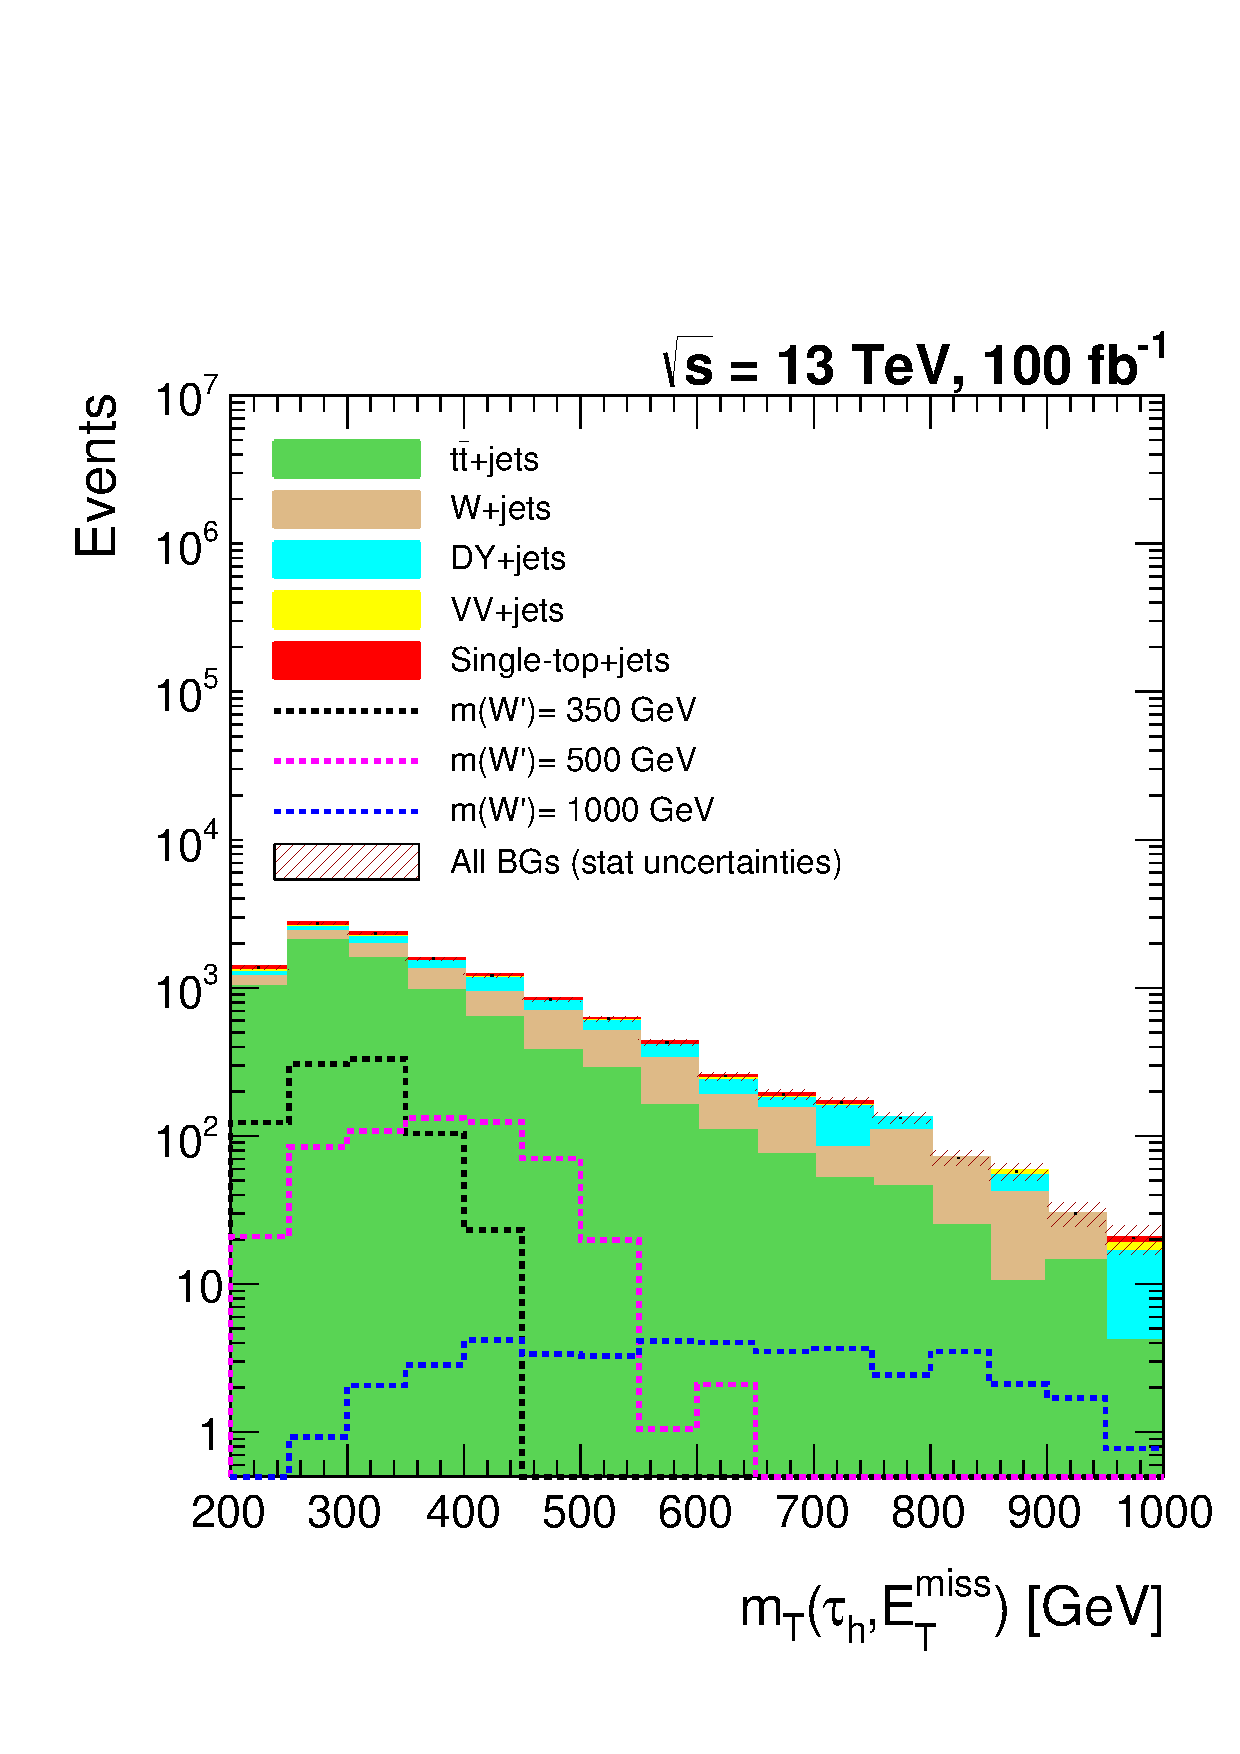
\includegraphics[width=0.5\textwidth]{mT_tauMet.pdf}
 \end{center}
 \caption{Distribución de $m_{T}(\tau_{h},E^{\text{miss}}_{T})$ después de la aplicación de todos los criterios de selección. Los backgrounds se acumulan mientras las señales están superpuestas. Todos los procesos incluidos están normalizados para la sección transversal de producción y la luminosidad de ($100\text{ fb}^{-1}$).}
 \label{Fig:mTstacked}
 \end{figure} 
%

\section{Resultados}\label{sec:results}

Las tablas \ref{tab:cutefficiencySMnew} y \ref{tab:cutefficiencynw} muestran la eficiencia de la selección cinemática basados en la tabla~\ref{tab:selections} y significancia de $100$ fb$^{-1}$ de luminosidad. Se encuentra que la significancia se incrementa con la masa de $W'$ de $200$ GeV a $400$ GeV debido al aumento de la energía faltante en estado final. También se puede notar que el rango de masas de $250$ a $500$ GeV se puede comprobar  usando $100$ fb$^{-1}$ de luminosidad y a nivel de $5\sigma$ cuando $g'_q=g'_\tau=0.1$.

En la figura~\ref{Fig:limits} se muestra una sensitividad proyectada del LHC a $13$ TeV usando este análisis, para $30$, $300$ y $3000$ fb$^{-1}$ de luminosidad en el plano $g'_q-m_{W'}$ superponiendo los ajustes a $1\sigma$ a las medidas de $R(D)$ y $R(D^{*})$ para los diferentes valores de $g'_\tau$. La región por encima de las lines negras tiene una significancia  igual o mayor que $3\sigma$. Gran parte de la banda de mejor ajuste esta al alcance con los datos actuales y la mayor parte de la región restante lo debe estar al final del Run 4.
%
\begin{figure}
\begin{center}
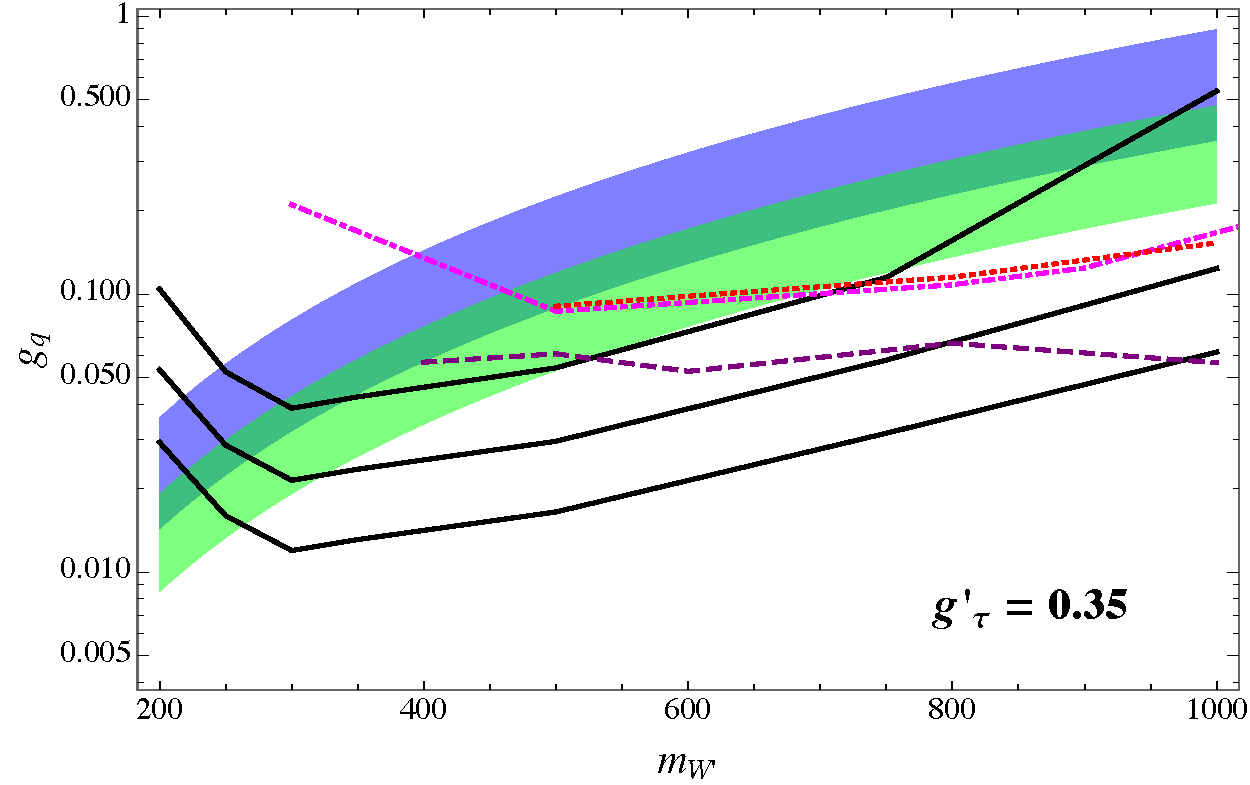
\includegraphics[width = 0.45 \textwidth]{gtau35e2.pdf}
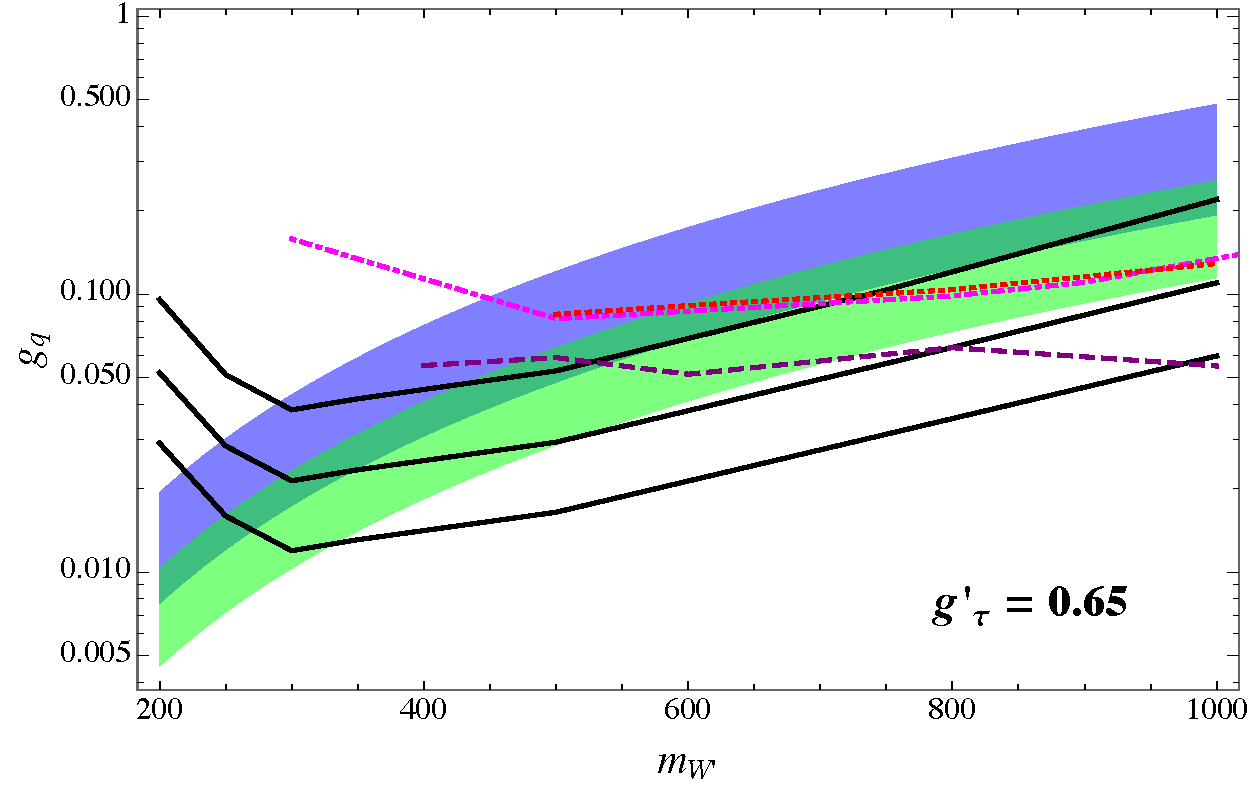
\includegraphics[width = 0.45 \textwidth]{gtau65e2.pdf}
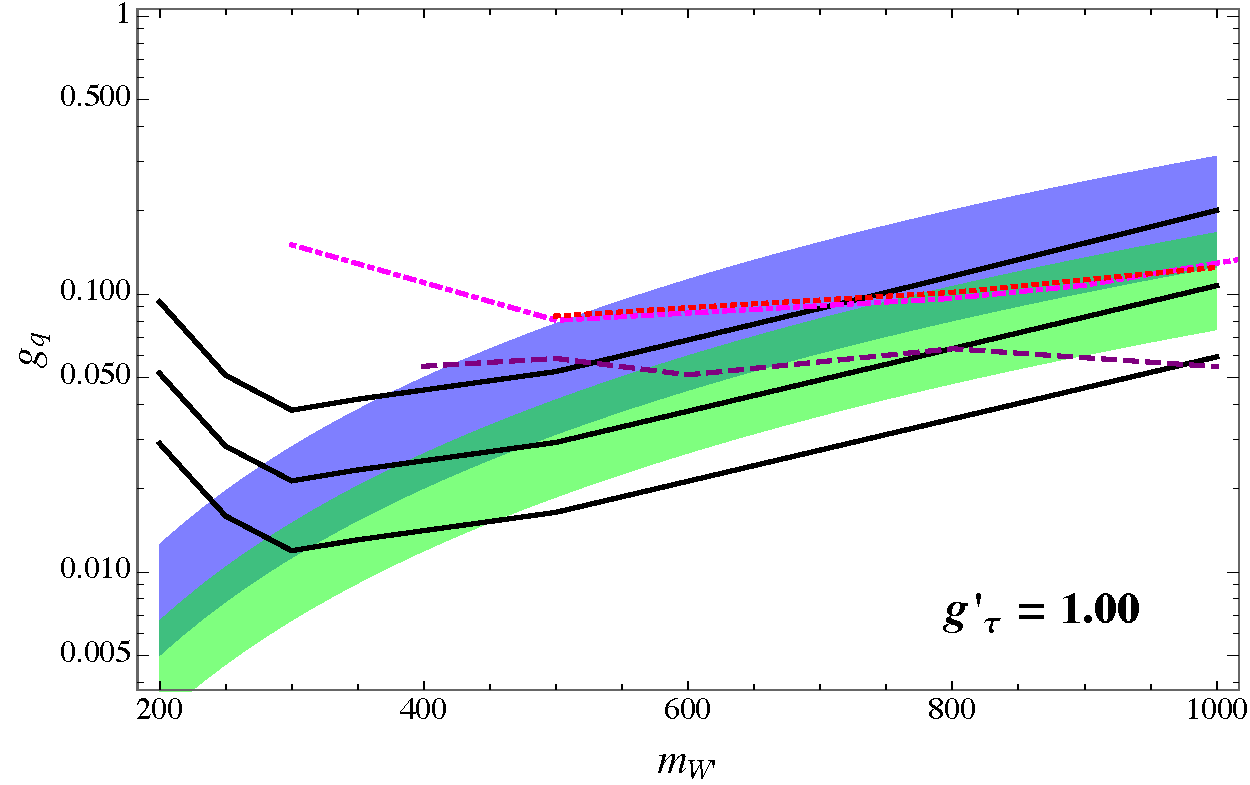
\includegraphics[width = 0.45 \textwidth]{gtau1e0.pdf}
\caption{Sensitividad proyectada a 3$\sigma$ en el acople a los quarks $g'_q$ como función de $m_{W'}$ para $g'_\tau = 0.35\,,0.65\,,1$ en el LHC a 13 TeV y $\mathcal{L}=30\,, 300\,, 3000\, \text{fb}^{-1}$ (curva negra solida) superpuesto con la banda a 1$\sigma$ explicando las medidas de $R(D)$ (azul) and $R(D^\ast)$ (verde). También se muestra los límites inclusivos utilizados por ATLAS a 13 TeV (curva roja punteada) y CMS a 8 TeV (curva magenta punteada).}
\label{Fig:limits}
\end{center}
\end{figure}
%
Note que cuando $g'_{\tau}$ cae por debajo de $0.35$ se comienza a perder la sensitividad debido a los pequeños branching a leptones, y los límites proyectados desaparecen por completo para la luminosidad máxima por debajo de aproximadamente $g'_{\tau} = 0.03$. Cuando $g'_{\tau}$ aumenta, mejora el alcance hasta que los branching a leptones se saturan al $100\%$. Más allá del punto de saturación, los límites no se verán afectados, pero las bandas que están de acuerdo con las anomalías en el mesón $B$ se moveran a valores inferiores de $g'_q$ para compensar. Es importante notar que los límites que se imponen están en los acoplamientos asumidos en la Eq.~\eqref{Eq:LagWp}, los cuales dependen de la teoría completa, podría tener un límite superior comparable a límites aplicados en este trabajo.

También se muestran los límites inclusivos (sin $b$-tag) de la búsqueda de ATLAS utilizando 13 TeV de energía y 36.1 $\text{fb}^{- 1}$ de datos~\cite{Aaboud:2018vgh}, la búsqueda de CMS usando 13 TeV y 35.9 $\text{fb}^{- 1}$~\cite{CMS:2018vff}, y la búsqueda de CMS a 8 TeV con 19.7 $\text{fb}^{- 1}$~\cite{Khachatryan:2015pua}. La búsqueda de 13 TeV de CMS proporciona límites más fuertes que nuestro análisis exclusivo para masas de más de 500 GeV y límites más débiles por debajo de eso. Los límites de ATLAS a 13 TeV, por otro lado, solo comienzan a competir con los límites exclusivos en aproximadamente 700 GeV. Tenga en cuenta que los límites de ATLAS parecen ser significativamente más débiles que los límites de CMS con la misma energía y proporcionan un alcance similar a los límites de CMS a 8 TeV.

\begin{table}[htbp]
\resizebox{17.3cm}{!} {
\begin{tabular}{clllllll}\hline
{} &       $p_T(\tau)$ &             $p_T(b)$ & $e/\mu$ veto & $E_T^{\text{miss}}$ &      $|\Delta \phi (\tau_h,E_T^{\text{miss}})|$ & $N/(\text{100 fb}^{-1})$ \\\hline
$t\bar{t}$    & $3.29 \pm 0.0056$  &   $49.8 \pm 0.087$ &   $71.8 \pm 0.11$ &  $12.4 \pm 0.096$ &  $24.8 \pm 0.36$& $7.41\times 10^{3}$ \\
mono-$t$   & $1.13 \pm 0.0035$ &   $40.4 \pm 0.0035$ &   $90.5 \pm 0.14$ &   $2.55 \pm 0.082$ &   $31.4 \pm 1.5$&$5.95\times 10^{2}$ \\
$W+j$    &   $2.97 \pm 0.0094$ &   $8.4 \pm 0.09$ &   $94.1 \pm 0.26$ &    $9.65 \pm 0.34$ &     $23 \pm 1.6$ &$2.61\times 10^{3}$\\
$Z+j$      &    $2.87 \pm 0.014$ &    $14.1 \pm 0.18$ &   $97.4 \pm 0.21$ &  $6.45 \pm 0.34$ &   $32.4 \pm 2.5$ &$1.37\times 10^{3}$\\
$WW$    & $0.575 \pm 0.0042$ &  $7.66 \pm 0.19$ &    $92.5 \pm 0.7$ &  $6.63 \pm 0.68$ &   $21.6 \pm 4.4$&$3.80\times 10^{1}$ \\
$WZ$     &    $0.638 \pm 0.0071$&  $11.9 \pm 0.36$ &   $93.2 \pm 0.82$ & $6.7 \pm 0.84$ &     $39 \pm 6.3$ &$1.08\times 10^{2}$\\
$ZZ$      &        $0.673 \pm 0.012$&   $17.8 \pm 0.67$ &    $92.7 \pm 1.1$ &     $6 \pm 1$ &   $65.6 \pm 8.4$&$1.77\times 10^{1}$ \\
\hline
&&&&&Total Background&$1.22\times 10^{4}$\\
\end{tabular} }
\caption {Selección de eficiencias en \% y el número total de eventos para 100 fb$^{-1}$ para los procesos de background del ME. Ver el texto y la tabla~\ref{tab:selections} para más detalles.}
\label{tab:cutefficiencySMnew}
\end{table}


\begin{table}[htbp]
\resizebox{17.3cm}{!} {
\begin{tabular}{cllllllll}\hline
{} &               $p_T(\tau)$ &             $p_T(b)$ & $e/\mu$ veto & $E_T^{\text{miss}}$ &      $|\Delta \phi (\tau_h,E_T^{\text{miss}})|$& $N/(\text{100 fb}^{-1})$& $\frac{S}{\sqrt{S+B}}$ \\\hline
200 GeV  &   $8.34 \pm 0.081$ &    $18.1 \pm 0.39$ &   $99.6 \pm 0.15$ &   $5.97 \pm 0.57$ &   $25.7 \pm 4.3$&$1.80\times 10^{2}$& 1.62 \\
250 GeV  &      $13.9 \pm 0.15$ &     $17.2 \pm 0.44$ &  $99.9 \pm 0.078$ &   $15.1 \pm 1$ &     $49 \pm 3.6$ &$5.98\times 10^{2}$&5.30\\
300 GeV  &    $18.3 \pm 0.24$ &     $17.4 \pm 0.56$ &   $99.9 \pm 0.13$ &   $28.6 \pm 1.6$ &   $69.2 \pm 3.1$& $1.06\times 10^{3}$&9.26\\
350 GeV  &    $22.2 \pm 0.27$ &     $17.1 \pm 0.52$ &   $99.7 \pm 0.19$ &   $37.6 \pm 1.6$ &   $67.8 \pm 2.5$&$8.88\times 10^{2}$&7.77 \\
500 GeV  &    $27.5 \pm 0.31$ &     $19.6 \pm 0.52$ &  $99.9 \pm 0.089$ &   $61.5 \pm 1.4$ &   $77.5 \pm 1.6$&$5.63\times 10^{2}$&5.00 \\
750 GeV  &    $31.5 \pm 0.34$ &     $21.7 \pm 0.54$ &   $99.7 \pm 0.16$ &   $79.1 \pm 1.2$ &   $82.4 \pm 1.2$&$1.55\times 10^{2}$&1.40 \\
1000 GeV &   $32.8 \pm 0.37$ &     $21.6 \pm 0.56$ &   $99.7 \pm 0.17$ &   $87.2 \pm 0.98$ &   $83.4 \pm 1.2$&$4.33\times 10^{1}$&0.39 \\\hline
\end{tabular} }
\caption {Selección de eficiencias en \%, y el número total de eventos y significancia para 100 fb$^{-1}$ para la señal en el rango de masas $M_{W'}$ y $g'_q=g'_\tau=0.1$. Ver el texto y la tabla~\ref{tab:selections} para más detalles.}
\label{tab:cutefficiencynw}
\end{table}
%
